\documentclass{beamer}
\date{\today}
\title{Multi-Agent Path Finding Visualization}
\author{Yihao Liu}

\begin{document}

\begin{frame}
  \titlepage
\end{frame}

\begin{frame}
\frametitle{Initial State of Agent 1}
The circles are available nodes, they are connected by edges (lines), and the squares (or walls) are obstacles.
\begin{figure}
\centering
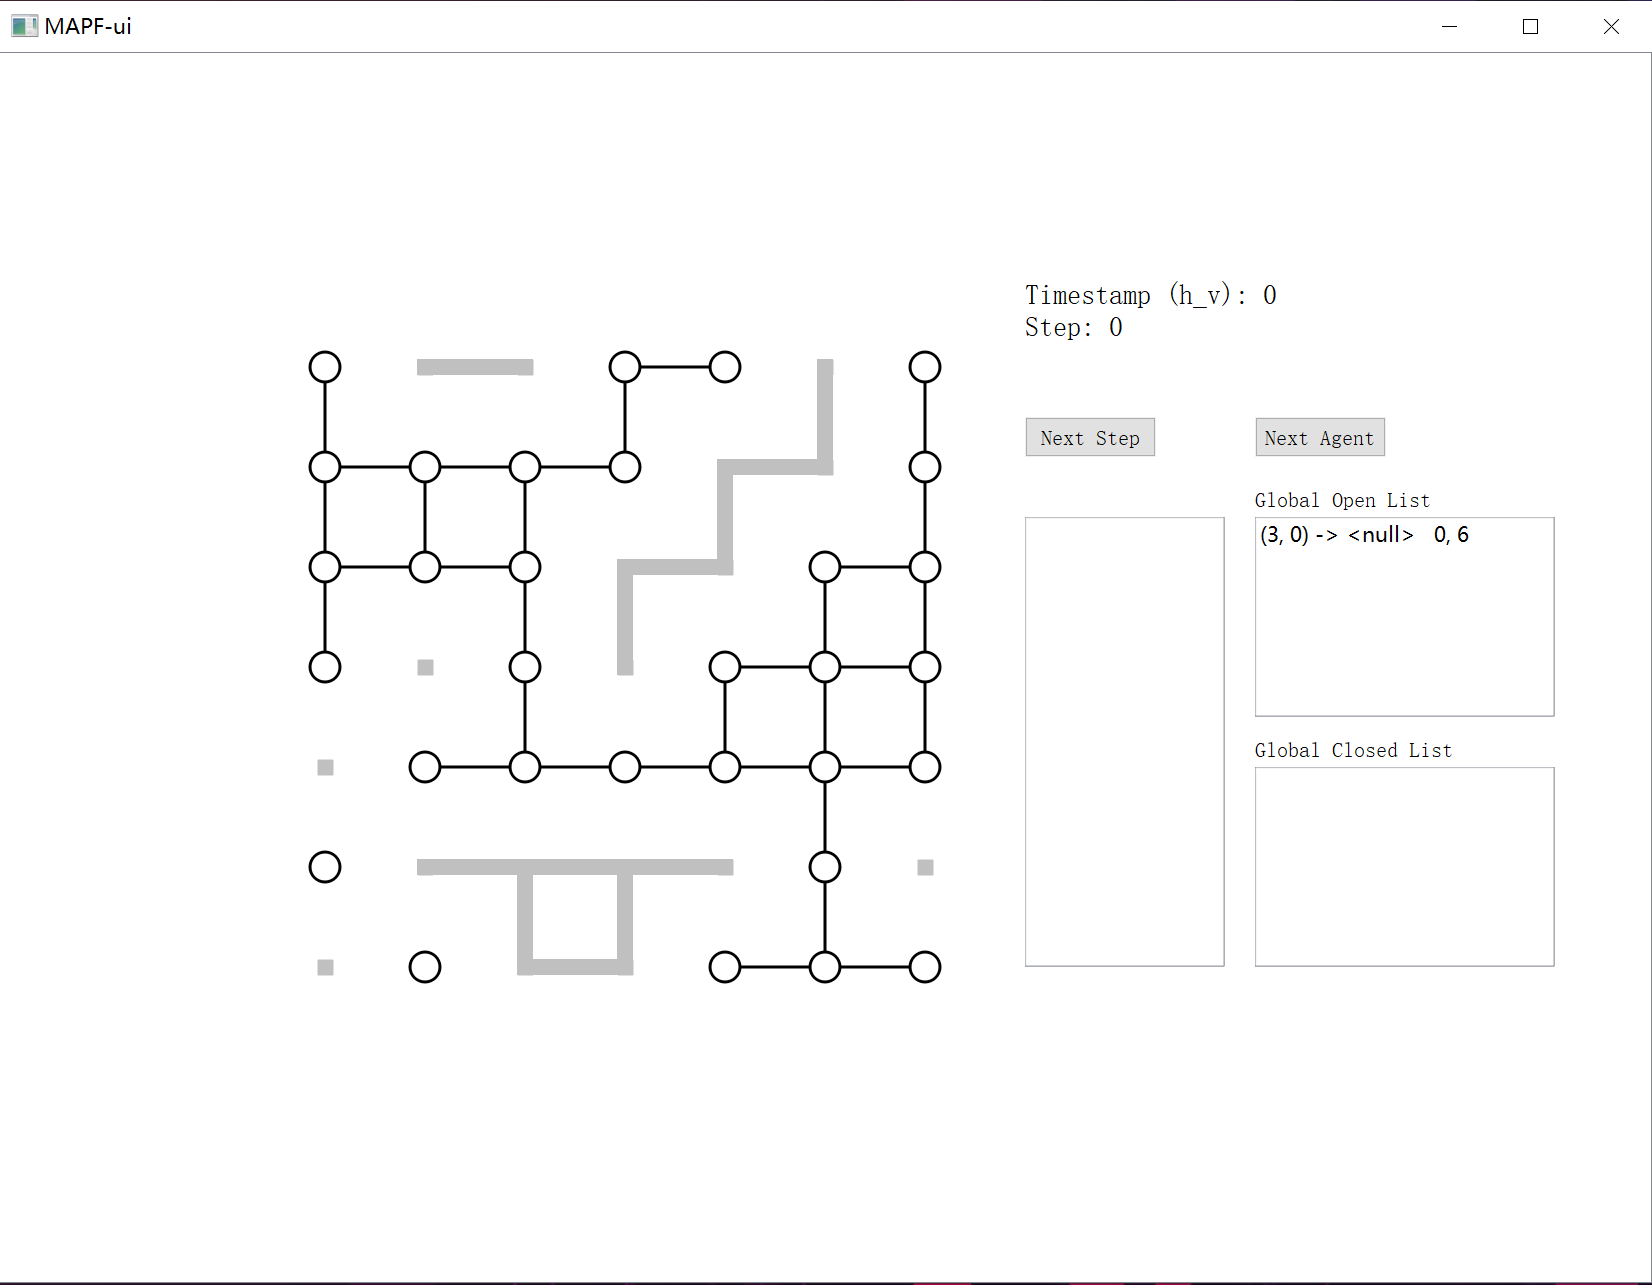
\includegraphics[width=0.8\textwidth]{1.png}
\end{figure}
\end{frame}

\begin{frame}
\frametitle{First Step of Agent 1}
The location of the current agent is marked in blue with a dot inside it.
\begin{figure}
\centering
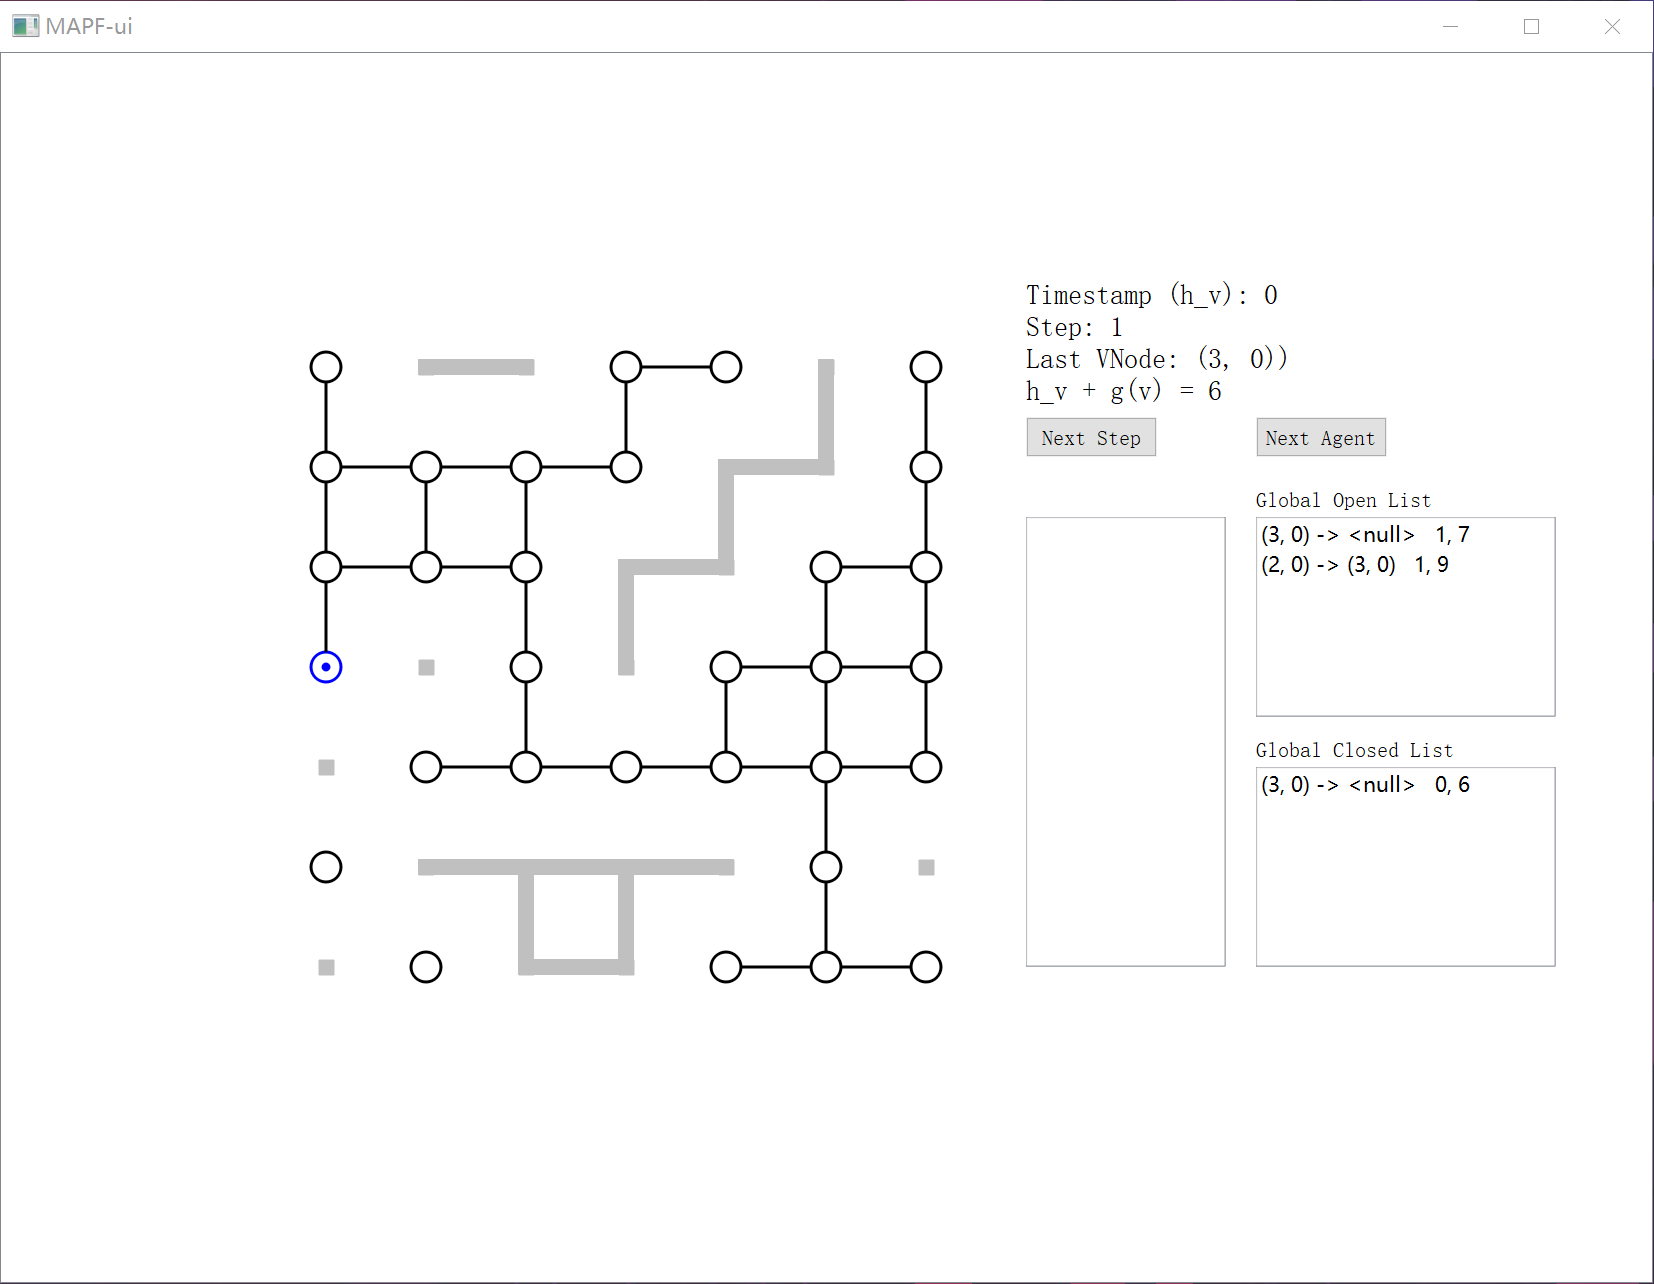
\includegraphics[width=0.8\textwidth]{2.png}
\end{figure}
\end{frame}

\begin{frame}
\frametitle{Last Step of Agent 1}
The path of the current agent is also marked in blue.
\begin{figure}
\centering
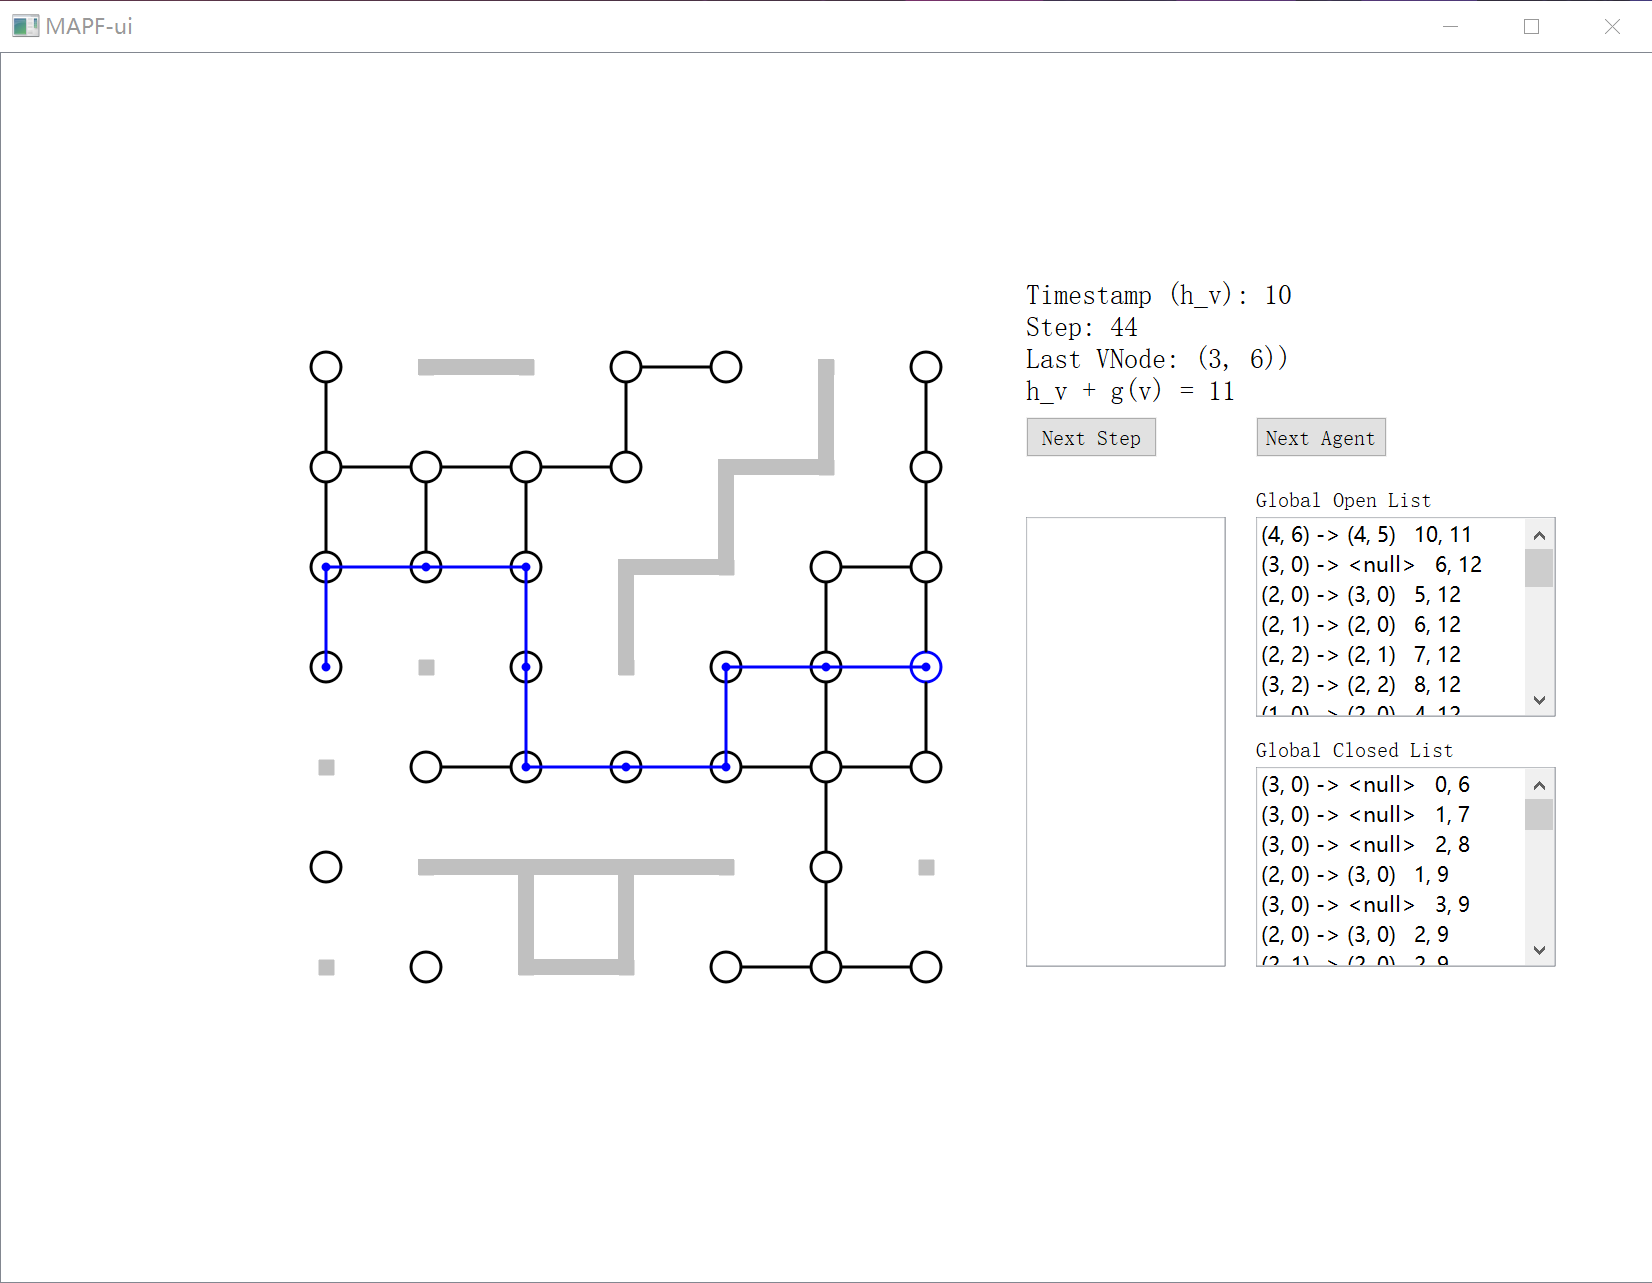
\includegraphics[width=0.8\textwidth]{3.png}
\end{figure}
\end{frame}

\begin{frame}
\frametitle{Initial State of Agent 2}
The constraints at the current timestamp are marked in red. At timestamp 0, they are the starting node and first edge of Agent 1.
\begin{figure}
\centering
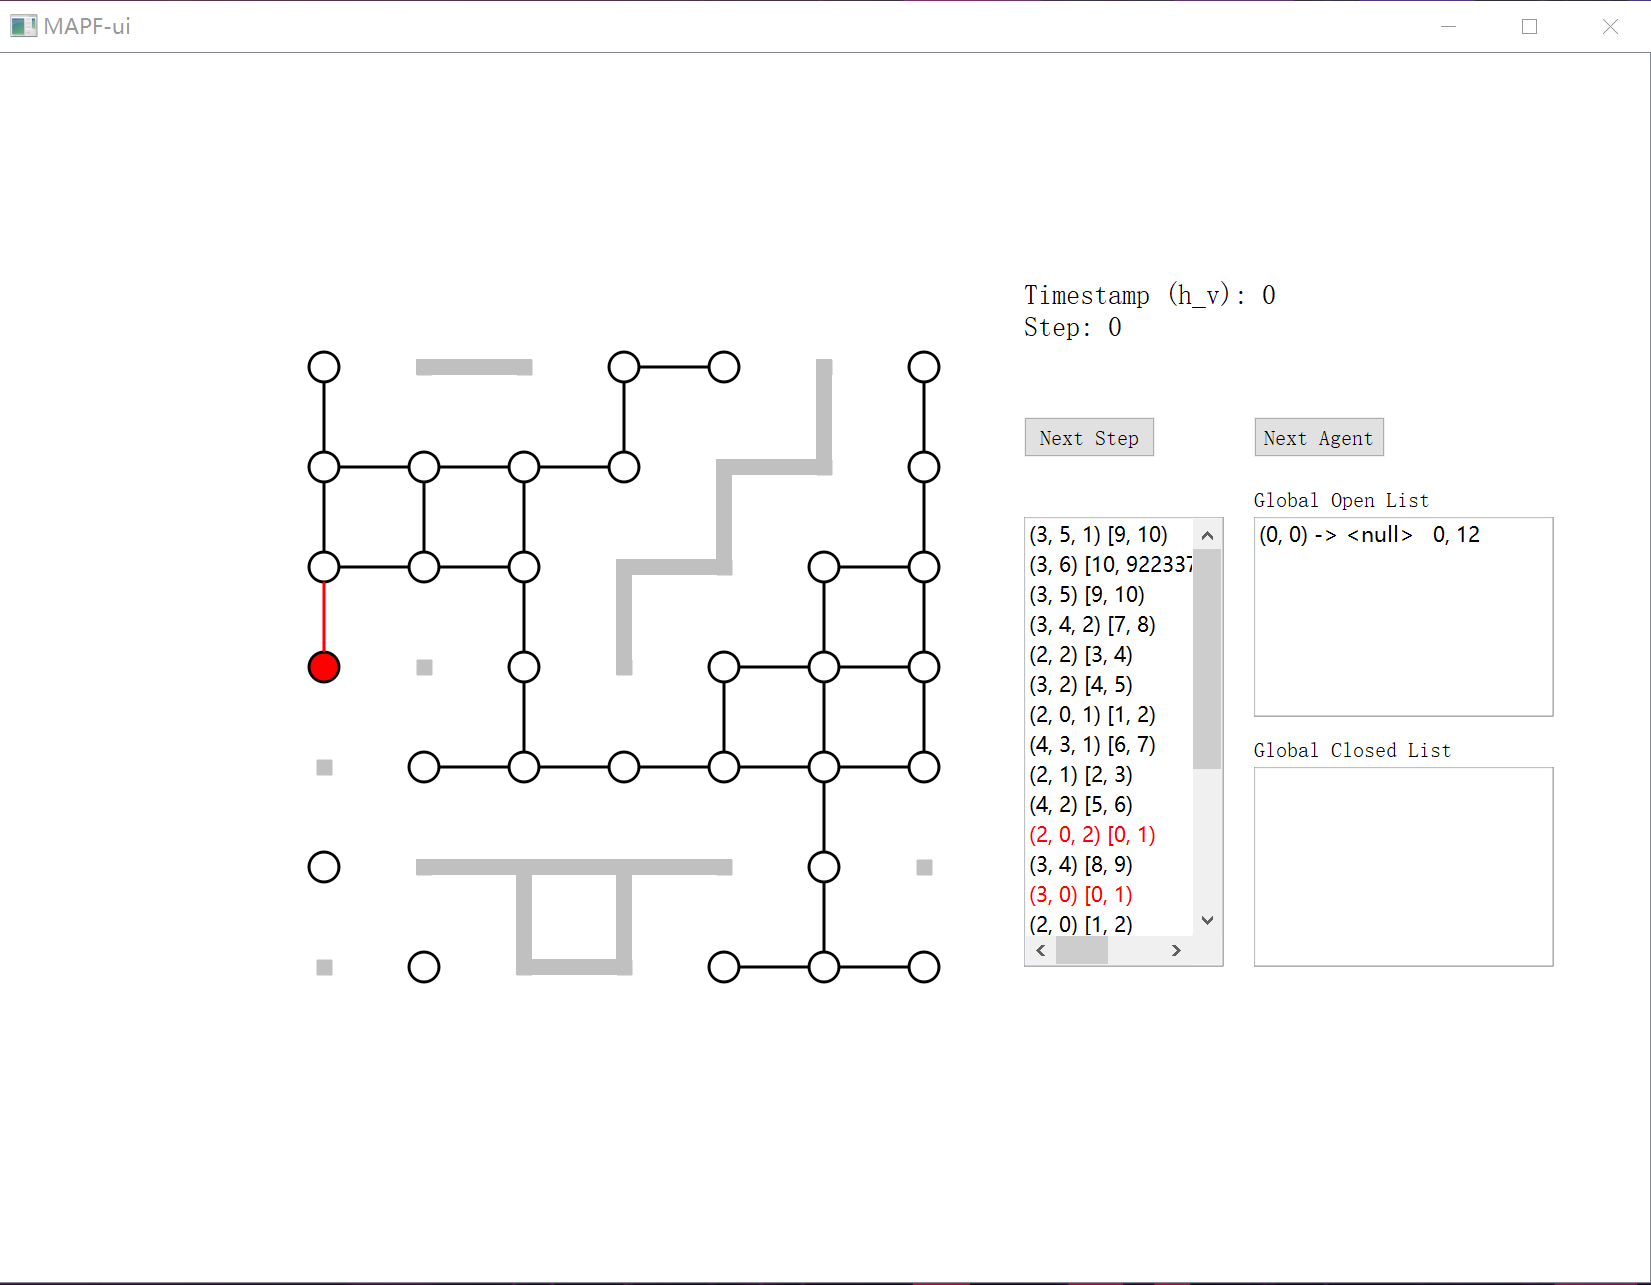
\includegraphics[width=0.8\textwidth]{4.png}
\end{figure}
\end{frame}

\begin{frame}
\frametitle{First Step of Agent 2}
Note that in the list in left all constraints are listed, in which red means that it's effective currently.
\begin{figure}
\centering
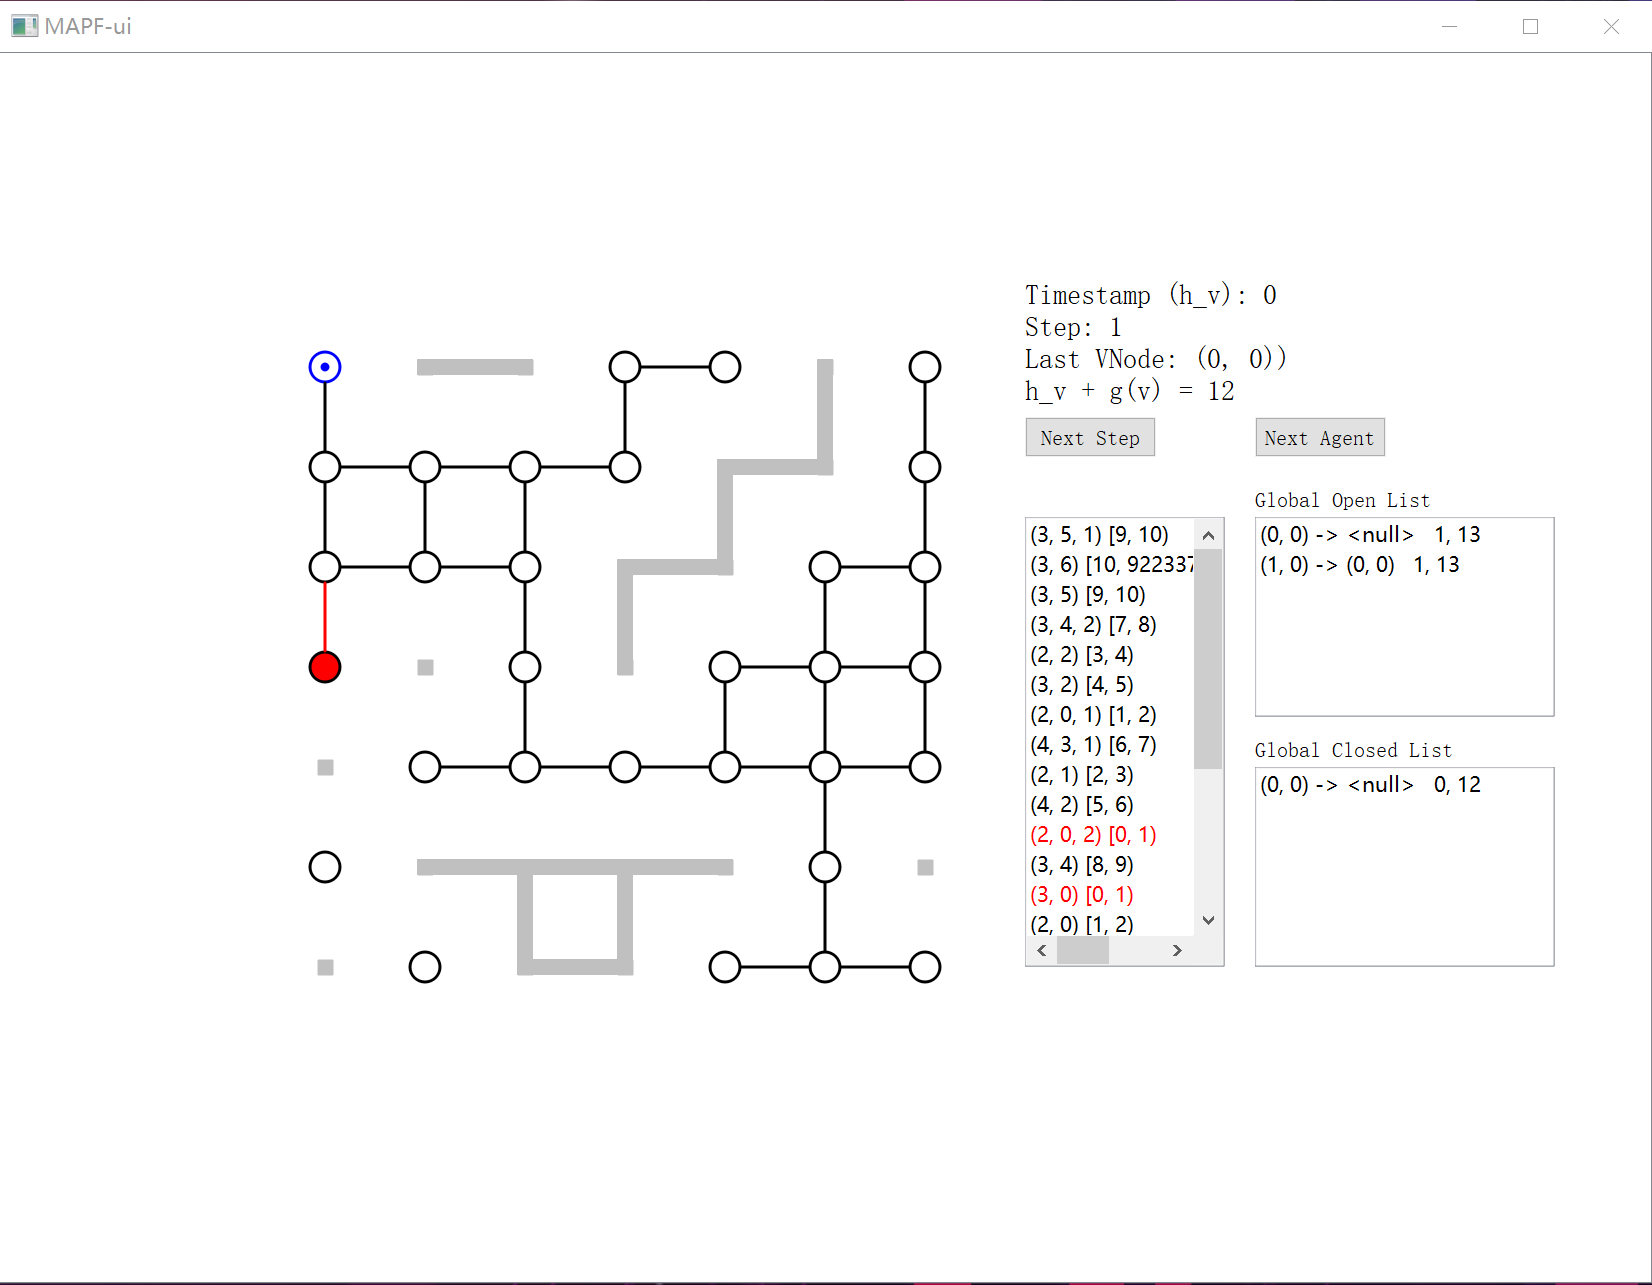
\includegraphics[width=0.8\textwidth]{5.png}
\end{figure}
\end{frame}

\begin{frame}
\frametitle{Middle Step of Agent 2}
After some time the current constraints may change.
\begin{figure}
\centering
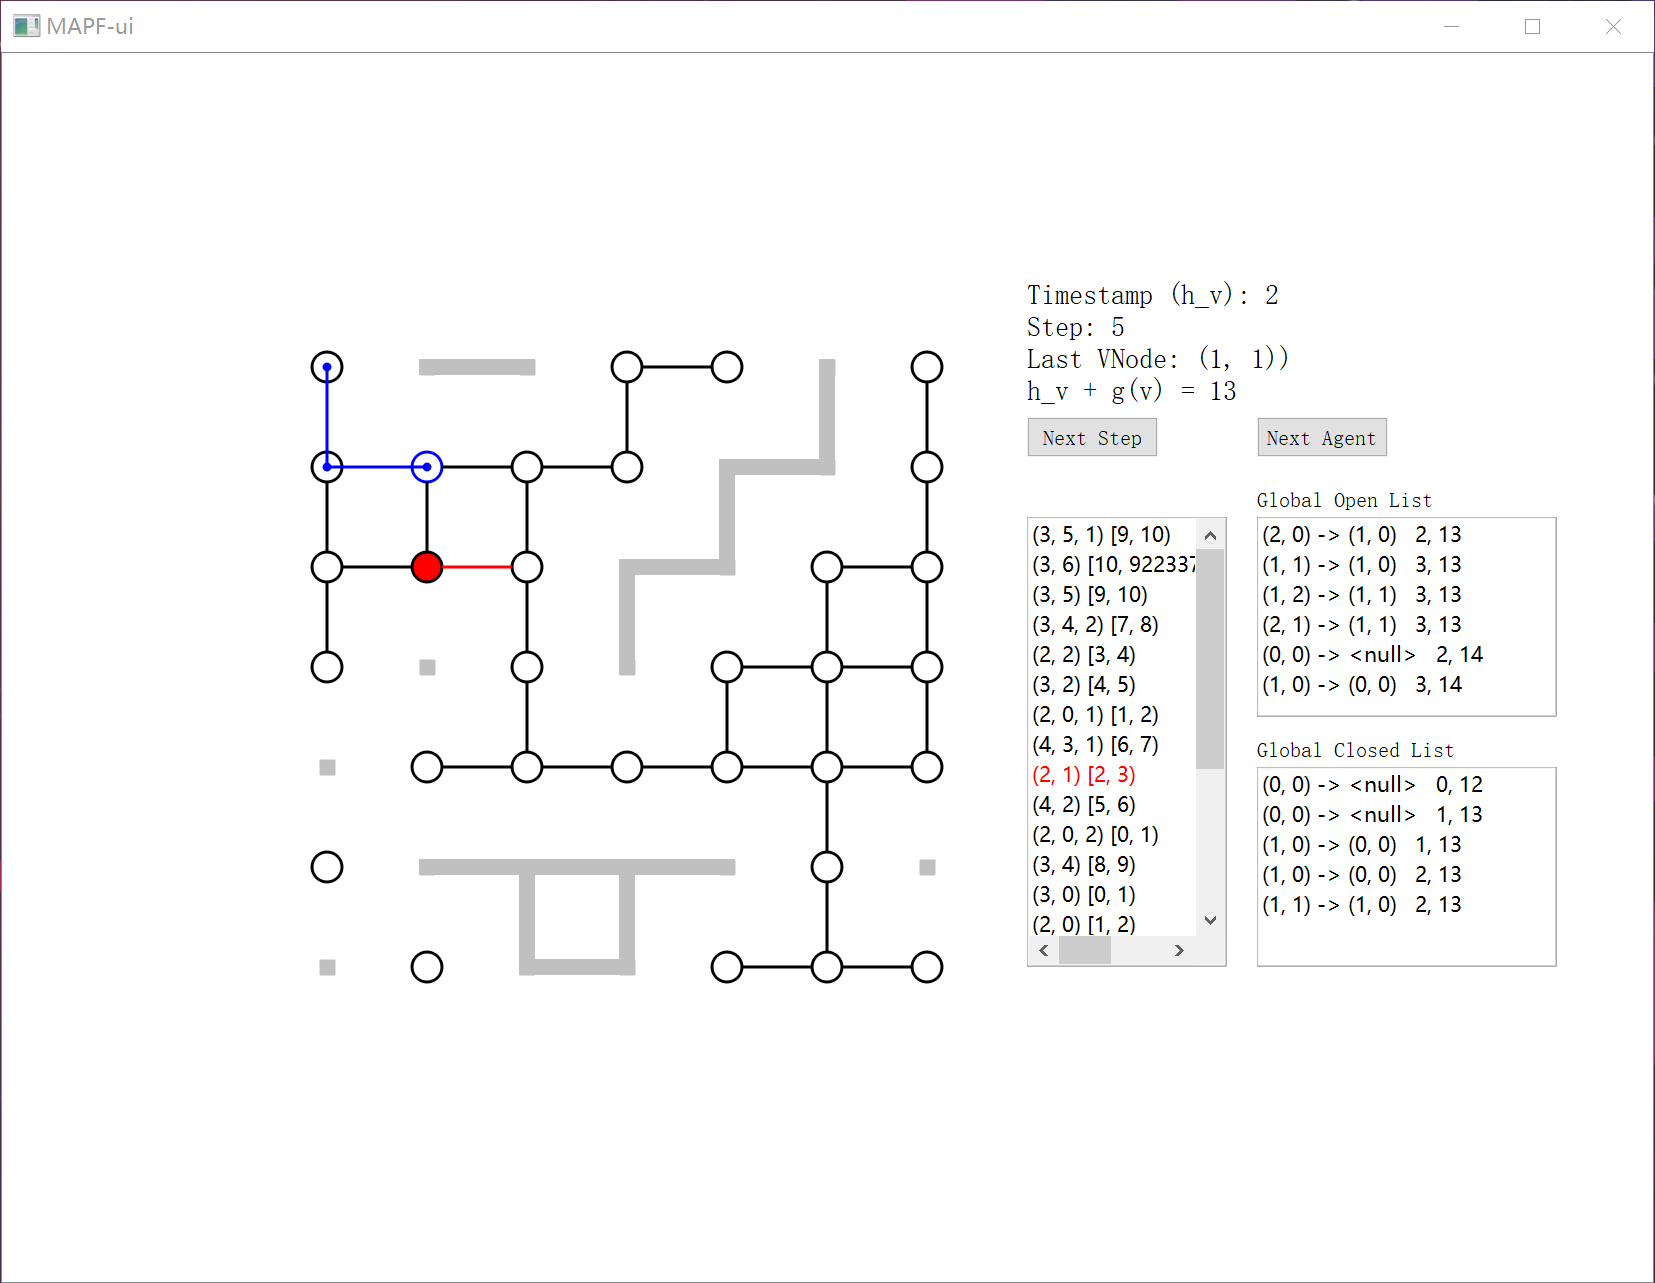
\includegraphics[width=0.8\textwidth]{6.png}
\end{figure}
\end{frame}

\begin{frame}
\frametitle{Last Step of Agent 2}
Note that in the two lists in right, the open and closed list can be viewed.
\begin{figure}
\centering
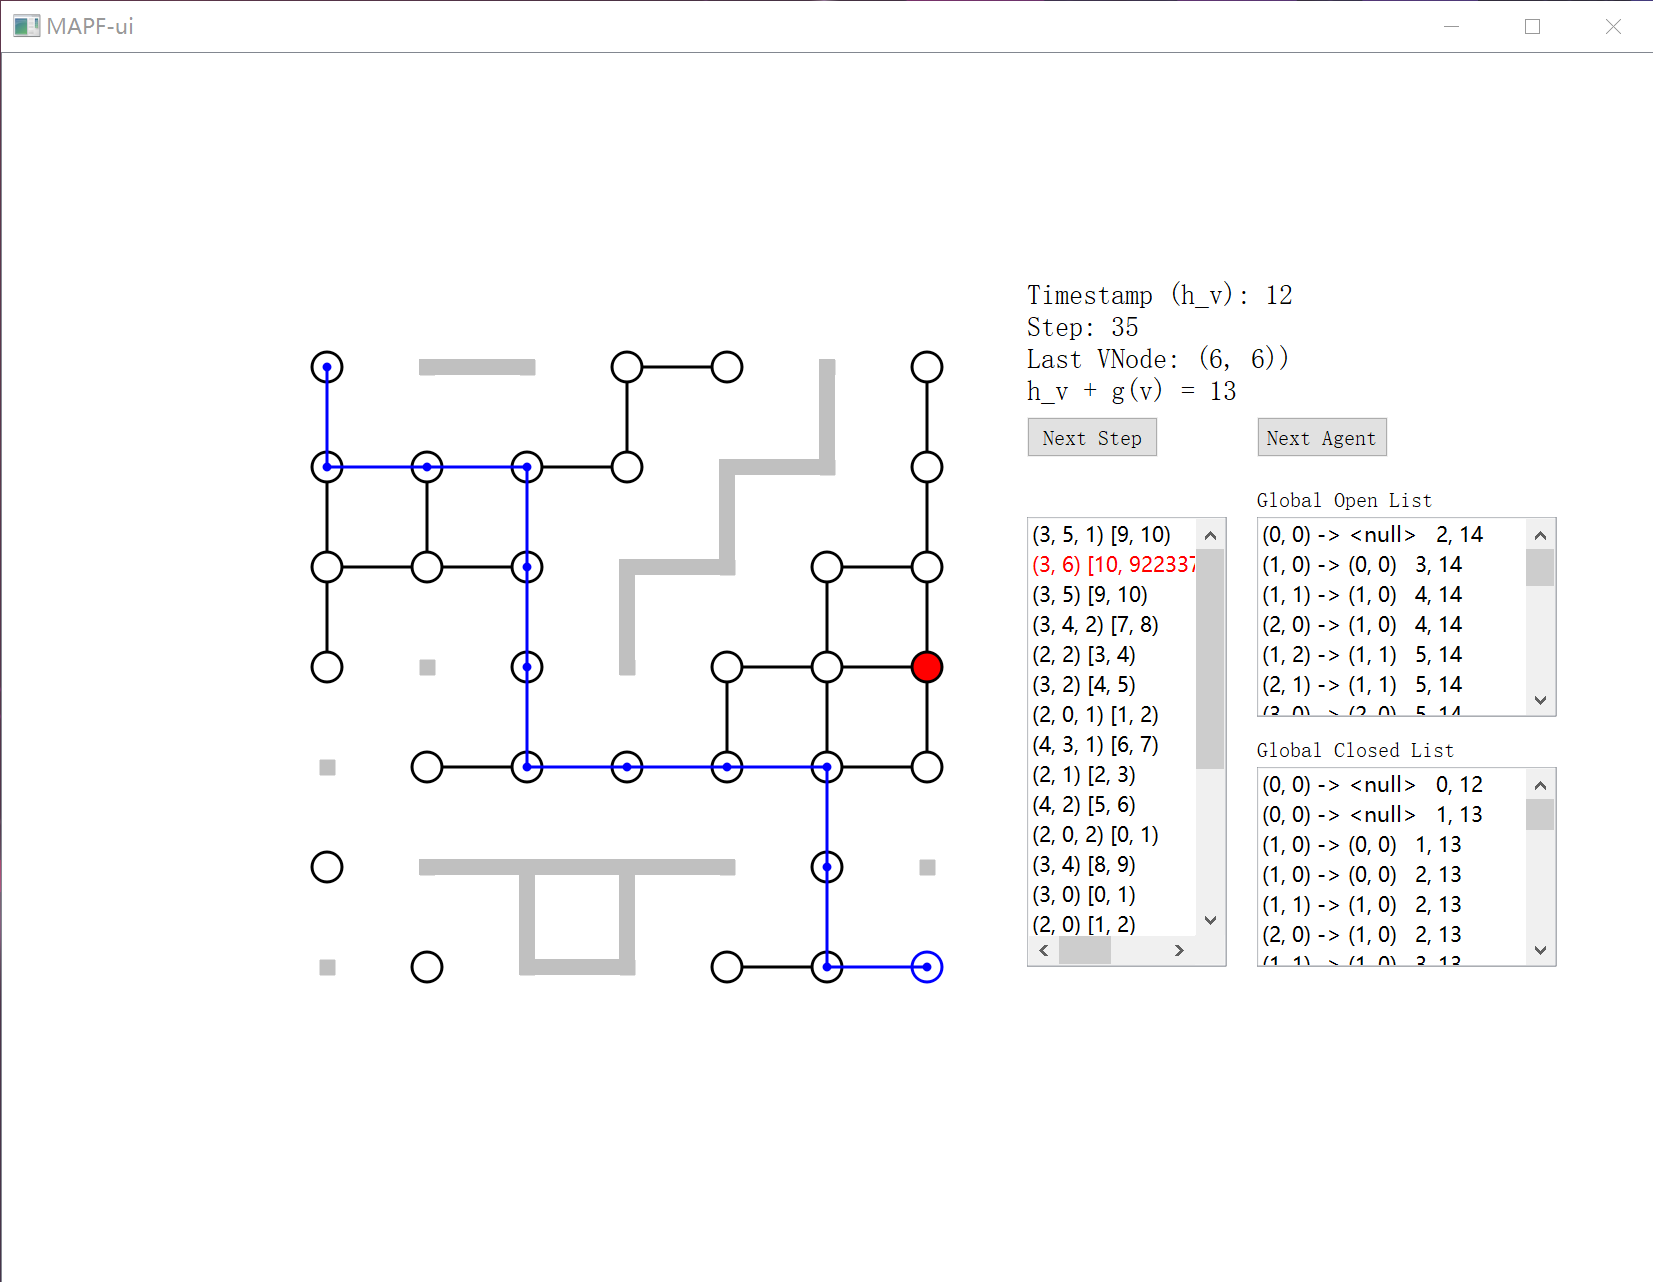
\includegraphics[width=0.8\textwidth]{7.png}
\end{figure}
\end{frame}

\end{document}

